The aim of this exercise is to generate the independent, discrete random variable $X_{i}$ having probability mass function 
\begin{equation}
    P\{X=x_{j}\} =p_{j},   j=0,1,...,\Sigma_{j}p_j=1
\end{equation}
To accomplish this, we assume, we have access to random number $U_{i}$ which is uniformly distributed over $(0,1)$ and finally transform $U_{i}$ to $X_{i}$. In this exercise we generated uniform random variables and we compared the results obtained in simulation with expected results with using histograms and tests.\\
\subsection{Geometric distribution}
first part of the exercise, Geometric distribution which is given by 
\begin{equation}
    F(n)=P(X\leq n)=1-(1-p)^n
\end{equation}
Where $X=\lfloor{(\frac{\log(U)}{\log(1-p)})}\lfloor+1$ with value of $p = 0.1$ is implemented and simulated for 10000 outcomes that shows in figure 4.\
\begin{center}
    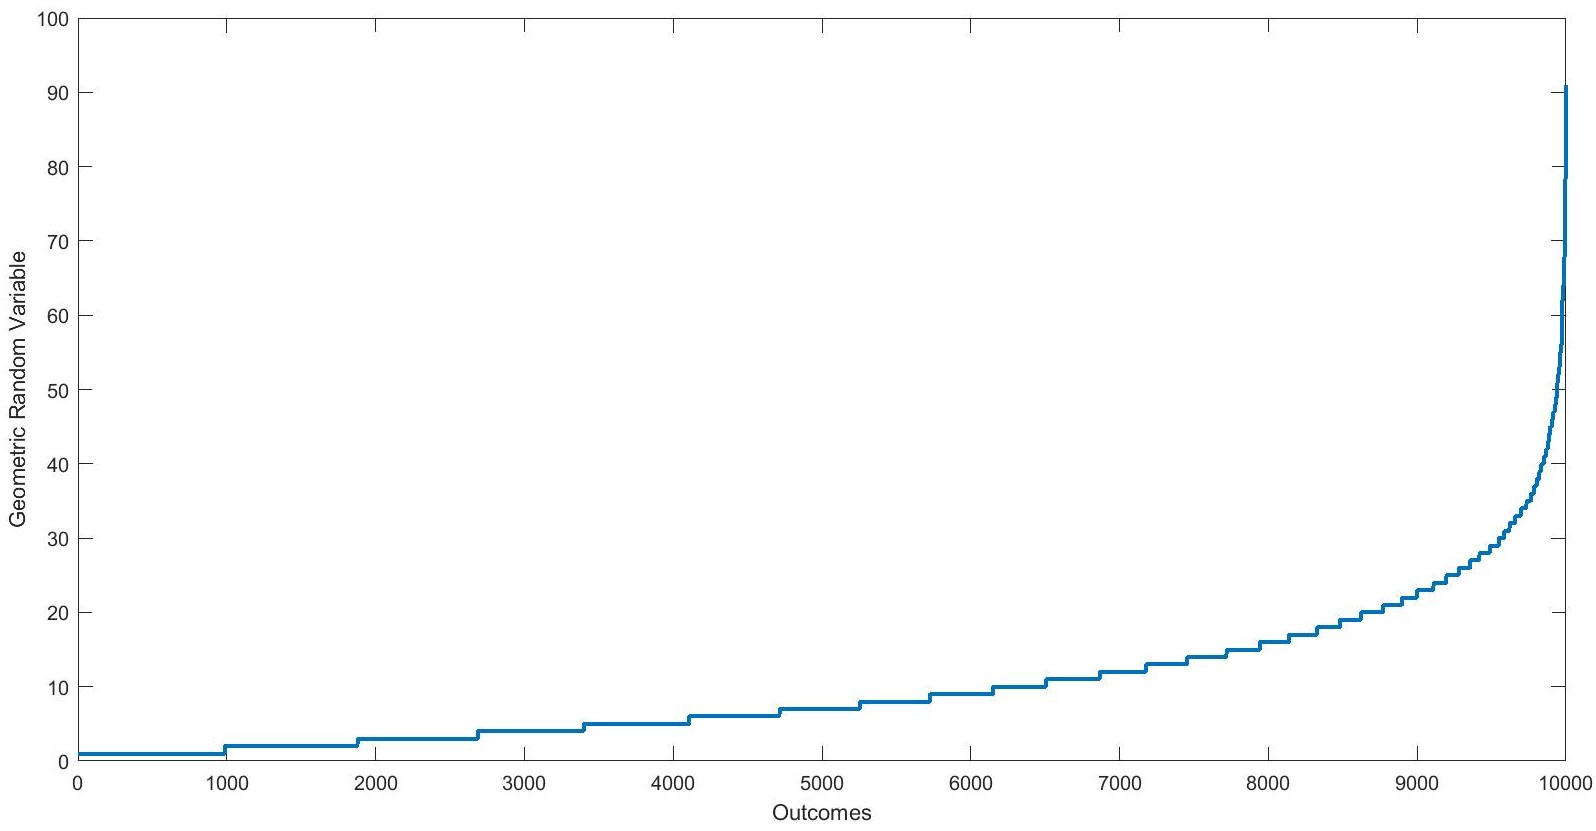
\includegraphics[scale=0.3]{Figures/figure2_1.jpg}\\
    \figuretitle{Figure 4:Geometric random variables for 10000 outcomes .}
\end{center}\\
\subsection{Simulate the 6 point distribution}

\begin{table}[h!]
\centering
\caption{6-point distribution.}
\label{summstats}
\begin{tabular}{|l|c|c|c|c|c|c|c|}
\hline
    X & 1 & 2 & 3 & 4 & 5 & 6  \\ \hline
    P_i & 7/48 & 5/48 & 1/8 & 1/16& 1/8 & 5/16 \\  \hline
\end{tabular}
\end{table}\\
\\
Figure 5 shows generating random variables and their histograms by By applying a direct(crude) method, rejection method and Alias method.\\
\begin{center}
    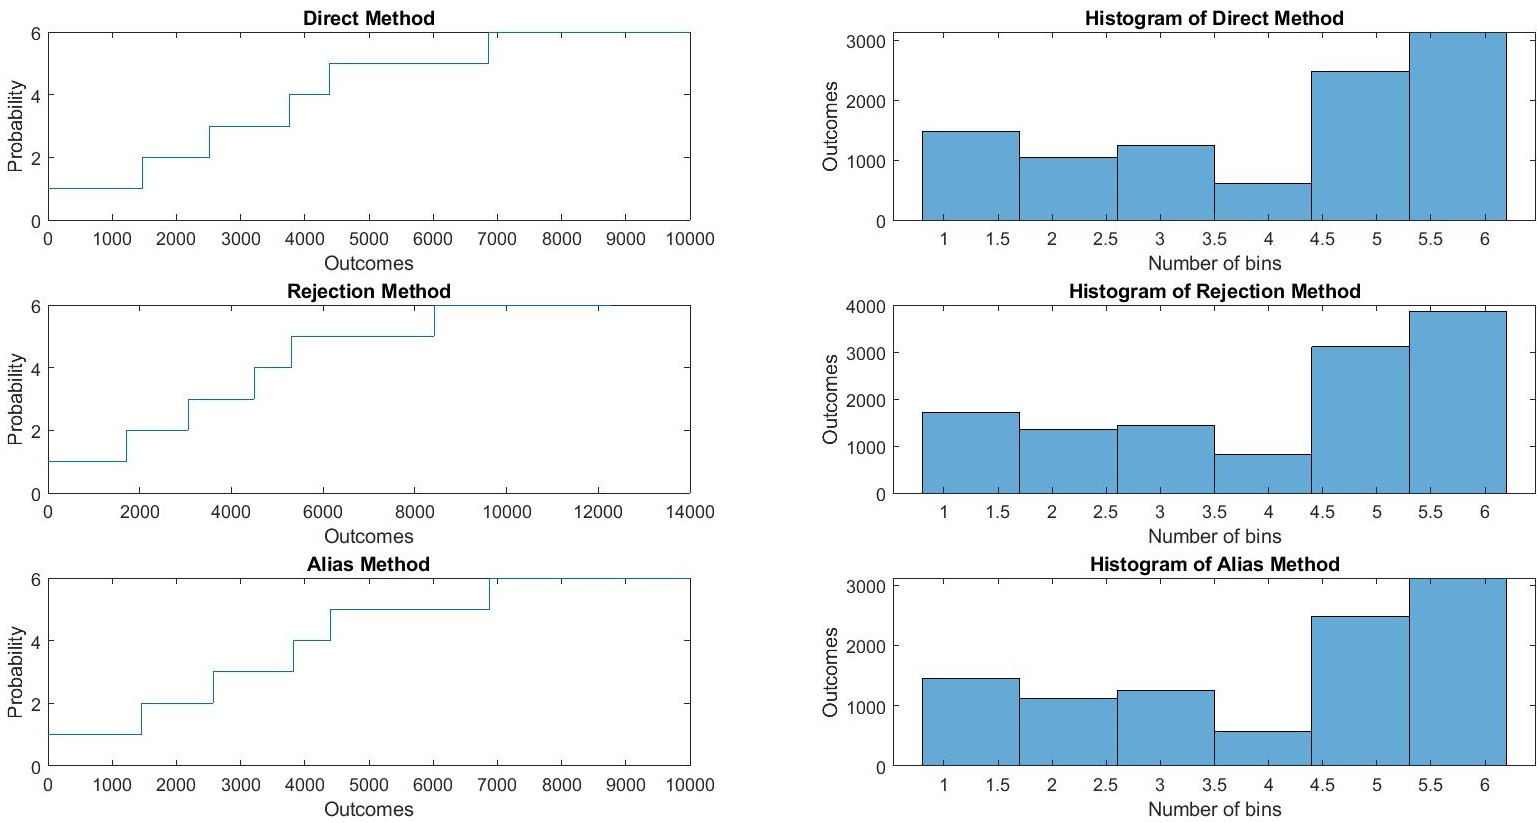
\includegraphics[scale=0.3]{Figures/figure2_2.jpg}\\
    \figuretitle{Figure 5: Different method for generating random variables and their histograms .}
\end{center}\\
\\Table2 presents result of  testing of generated uniform random variables with different methods .
\begin{table}[h!]
\centering
\caption{Testing of generated uniform random variables with different method .}
\label{summstats}
\begin{tabular}{|l|c|c|c|}
\hline
\textbf{Test}  & \multicolumn{1}{l|}{\textbf{Crude Method}} & \multicolumn{1}{l|}{\textbf{Rejection Method}}& \multicolumn{1}{l|}{\textbf{Alias Method}} \\ \hline

    $\chi^2$ Test & 1 & 1 & 1  \\ \hline
    KS Test & 1 & 1 & 1 \\  \hline
    Run Test & 0 & 1 & 1  \\ \hline
    CC Test & 1 & 1 & 1 \\  \hline
\end{tabular}
\end{table}\\
\\



